\documentclass[11pt,a4paper]{article}

% =========================================================================
% PAKET-PAKET UTAMA
% =========================================================================
\usepackage[utf8]{inputenc}
\usepackage[T1]{fontenc}
\usepackage{lmodern}
\usepackage[indonesian]{babel}
\usepackage{amsmath,amssymb,amsfonts,amsthm}
\usepackage{bm}              % Notasi tebal untuk vektor & matriks
\usepackage{geometry}
\geometry{top=2.5cm, bottom=2.5cm, left=2.5cm, right=2.5cm}
\usepackage{graphicx}
\usepackage{booktabs}        % Tabel profesional
\usepackage{tabularx}
\usepackage{microtype}
\usepackage{tikz}            % Diagram skematis
\usetikzlibrary{matrix,decorations.pathreplacing,calc,positioning,arrows.meta}
\usepackage{xcolor}
\usepackage{mdframed}        % Kotak highlight untuk pembuktian/definisi
\usepackage{caption}
\usepackage{subcaption}
\usepackage{hyperref}
\hypersetup{
    colorlinks=true,
    linkcolor=blue!70!black,
    citecolor=blue!70!black,
    urlcolor=blue!70!black,
    pdfencoding=auto,
    psdextra
}
\pdfstringdefDisableCommands{%
  \def\boldsymbol#1{#1}%
  \def\bm#1{#1}%
  \def\mathbf#1{#1}%
}

% Makro sitasi standar
\newcommand{\citep}[2][]{(Rasmussen \& Williams, 2006\if\relax\detokenize{#1}\relax\else, #1\fi)}
\newcommand{\citet}[2][]{Rasmussen \& Williams (2006\if\relax\detokenize{#1}\relax\else, #1\fi)}

% Pengaturan lingkungan matematika
\newtheorem{definisi}{Definisi}[section]
\newtheorem{teorema}{Teorema}[section]
\newtheorem{proposisi}{Proposisi}[section]
\newtheorem{catatan}{Catatan}[section]

% Path direktori gambar
\graphicspath{{figures/}}

% =========================================================================
% INFORMASI DOKUMEN (SEDERHANA SESUAI BIMBINGAN 02)
% =========================================================================
\title{
    \vspace{-1.2cm}
    \textbf{\Large BIMBINGAN TUGAS AKHIR \#3} \\[0.2em]
}
\begin{document}

\maketitle
\vspace{-0.6cm}

% =========================================================================
% BAGIAN 1: ANALISIS KETERDIFERENSIALAN MEAN-SQUARE & SPEKTRUM KERNEL
% =========================================================================
\section{Analisis Keterdiferensialan \textit{Mean-Square} dan Spektrum Kehalusan Kernel}
\label{sec:kernel_smoothness}

Melanjutkan fondasi regresi dan inferensi pada dokumen sebelumnya, bagian ini berfokus pada analisis analitik sifat kehalusan ruang fungsi (\textit{mean-square differentiability}) yang ditentukan oleh struktur matematis fungsi kovariansi $k(\mathbf{x}, \mathbf{x}')$.

\subsection{Perbandingan Analitik Jarak Linier $r$ vs Jarak Kuadratik $r^2$}

Diberikan dua titik input $\mathbf{x}, \mathbf{x}' \in \mathbb{R}^{D \times 1}$ dengan jarak Euclidean $r = \|\mathbf{x} - \mathbf{x}'\|_2 = \sqrt{(\mathbf{x} - \mathbf{x}')^T(\mathbf{x} - \mathbf{x}')}$. Perbedaan perlakuan terhadap $r$ menghasilkan sifat keterdiferensialan fungsi stokastik yang sangat kontras:

\begin{enumerate}
    \item \textbf{Kernel Squared Exponential (Berbasis $r^2$)}:
    \begin{equation}
    k_{\text{SE}}(r) = \sigma_f^2 \exp\left(-\frac{r^2}{2l^2}\right)
    \end{equation}
    Pada $r = 0$, turunan pertama terhadap jarak bernilai nol:
    \begin{equation}
    \left. \frac{d k_{\text{SE}}}{dr} \right|_{r=0^+} = \left. -\frac{\sigma_f^2 r}{l^2} \exp\left(-\frac{r^2}{2l^2}\right) \right|_{r=0^+} = 0
    \end{equation}
    Karena fungsi kovariansi analitik pada titik asal ($r=0$) dan memiliki turunan berhingga pada semua orde, proses Gaussian yang dihasilkan bersifat \textbf{terdiferensiasi tak hingga secara mean-square} ($C^\infty$). Realisasi sampel fungsi dari kernel ini sangat mulus (\textit{smooth}).

    \item \textbf{Kernel Exponential / Ornstein-Uhlenbeck (Berbasis $r$)}:
    \begin{equation}
    k_{\text{Exp}}(r) = \sigma_f^2 \exp\left(-\frac{r}{l}\right)
    \end{equation}
    Pada $r = 0$, turunan satu sisi menghasilkan nilai konstan non-nol:
    \begin{equation}
    \left. \frac{d k_{\text{Exp}}}{dr} \right|_{r=0^+} = -\frac{\sigma_f^2}{l} \neq 0
    \end{equation}
    Adanya sudut tajam (\textit{cusp}) pada $r = 0$ menyebabkan proses stokastik \textbf{tidak terdiferensiasi secara mean-square} ($C^0$). Sampel fungsi kontinu namun sangat kasar (\textit{jagged}), identik dengan lintasan Gerak Brown (\textit{Brownian motion}) 1D.
\end{enumerate}

\begin{figure}[h!]
\centering
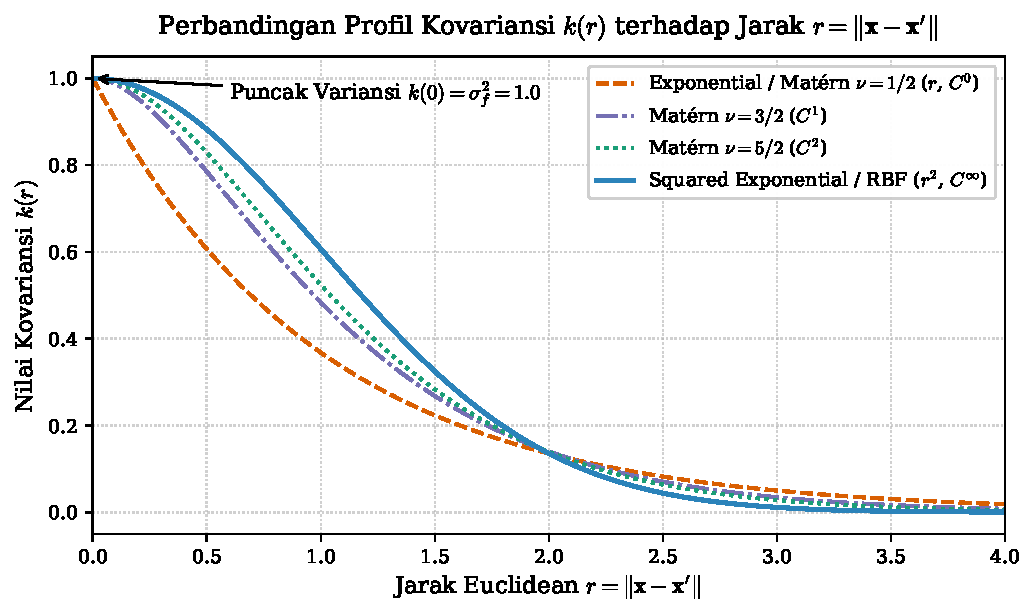
\includegraphics[width=0.75\textwidth]{fig1_kernel_profiles.pdf}
\caption{Profil kurva kovariansi $k(r)$ terhadap jarak Euclidean $r = \|\mathbf{x}-\mathbf{x}'\|$ ($l=1.0, \sigma_f^2=1.0$).}
\label{fig:kernel_profiles}
\end{figure}

\subsection{Keluarga Matérn sebagai Spektrum Ruang Fungsi Sobolev}

Keluarga kernel Matérn memfasilitasi parameterisasi eksplisit terhadap derajat keterdiferensialan proses stokastik melalui parameter $\nu > 0$:
\begin{equation}
k_{\text{Matérn}}(r) = \sigma_f^2 \frac{2^{1-\nu}}{\Gamma(\nu)} \left(\frac{\sqrt{2\nu}\,r}{l}\right)^\nu K_\nu\left(\frac{\sqrt{2\nu}\,r}{l}\right)
\end{equation}
Proses stokastik $f(\mathbf{x})$ dengan kernel Matérn bersifat $k$-kali terdiferensiasi \textit{mean-square} jika dan hanya jika $\nu > k$. Dengan memilih $\nu = p + 1/2$ ($p \in \mathbb{N}$), diperoleh spektrum kehalusan analitik:
\begin{itemize}
    \item $\nu = 1/2$ ($C^0$, Kasar): $k_{1/2}(r) = \sigma_f^2 \exp\left(-\frac{r}{l}\right) \equiv k_{\text{Exp}}(r)$
    \item $\nu = 3/2$ ($C^1$, Sekali Terdiferensiasi): $k_{3/2}(r) = \sigma_f^2 \left(1 + \frac{\sqrt{3}r}{l}\right) \exp\left(-\frac{\sqrt{3}r}{l}\right)$
    \item $\nu = 5/2$ ($C^2$, Dua Kali Terdiferensiasi): $k_{5/2}(r) = \sigma_f^2 \left(1 + \frac{\sqrt{5}r}{l} + \frac{5r^2}{3l^2}\right) \exp\left(-\frac{\sqrt{5}r}{l}\right)$
    \item Limit $\nu \to \infty$ ($C^\infty$, Mulus Tak Hingga): $\lim_{\nu \to \infty} k_{\text{Matérn}}(r) = k_{\text{SE}}(r)$
\end{itemize}

\begin{figure}[h!]
\centering
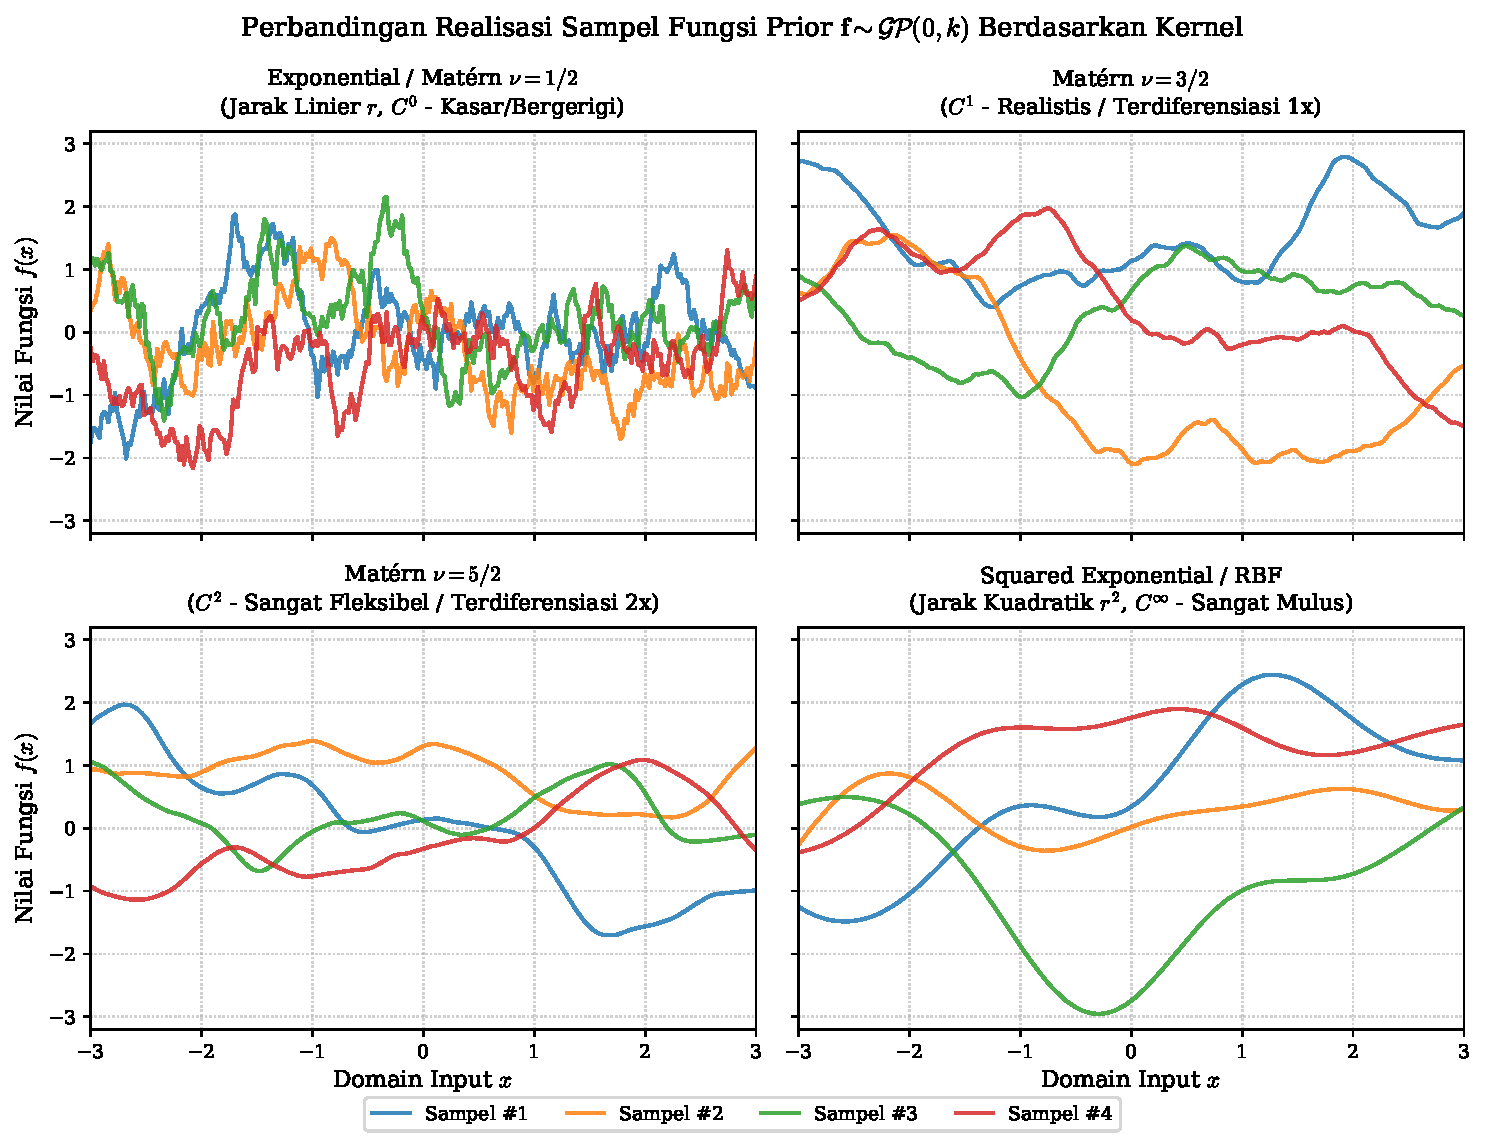
\includegraphics[width=0.95\textwidth]{fig2_sample_paths_kernels.pdf}
\caption{Realisasi sampel fungsi prior $\mathbf{f} \sim \mathcal{GP}(0, k)$ memperlihatkan spektrum kehalusan dari $C^0$ hingga $C^\infty$.}
\label{fig:sample_paths}
\end{figure}

\subsection{Analisis Pengaruh Hyperparameter Spasial}

Dua hyperparameter utama mengendalikan geometri realisasi fungsi:
\begin{enumerate}
    \item \textbf{Lengthscale ($l$)}: Mengontrol frekuensi spasial fluktuasi fungsi. Nilai $l$ yang kecil menghasilkan fungsi yang berosilasi cepat, sedangkan $l$ yang besar memaksa fungsi menjadi lebih kaku dan lambat berubah.
    \item \textbf{Signal Variance ($\sigma_f^2$)}: Mengatur rentang amplitudo simpangan vertikal terhadap mean.
\end{enumerate}

\begin{figure}[h!]
\centering
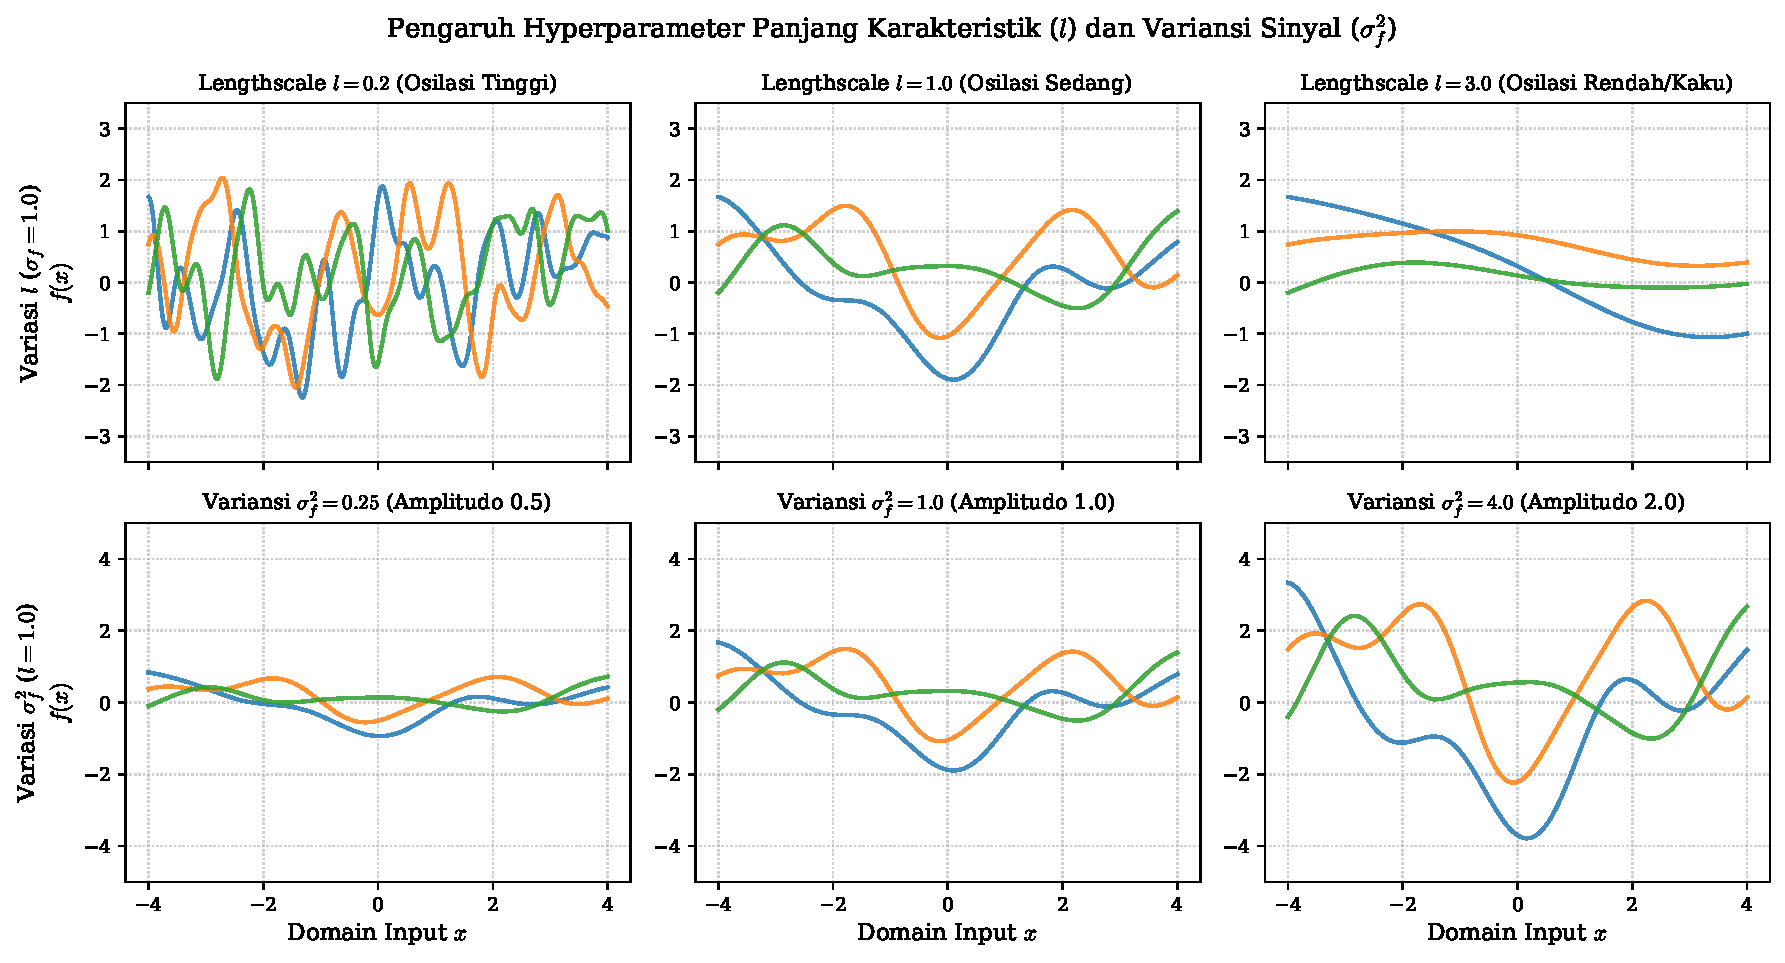
\includegraphics[width=0.95\textwidth]{fig3_hyperparameter_effects.pdf}
\caption{Simulasi efek hyperparameter: (Atas) Variasi \textit{lengthscale} $l \in \{0.2, 1.0, 3.0\}$; (Bawah) Variasi \textit{signal variance} $\sigma_f^2 \in \{0.25, 1.0, 4.0\}$.}
\label{fig:hyperparameter_effects}
\end{figure}

% =========================================================================
% BAGIAN 2: MEKANISME SAMPLING CHOLESKY
% =========================================================================
\section{Mekanisme Generatif dan Sampling Fungsi via Dekomposisi Cholesky}
\label{sec:cholesky_sampling}

Salah satu keunggulan utama dari perumusan \textit{Gaussian Process} adalah kemampuannya untuk membangkitkan realisasi fungsi konkret (\textit{function sampling}) dari distribusi ruang fungsi. Bagian ini menguraikan konsep fundamental, intuisi matematis, serta tahapan komputasi langkah demi langkah dari proses sampling tersebut.

\subsection{Motivasi Fundamental dan Masalah Generatif}

Secara fisik dan komputasional, sebuah komputer digital tidak dapat langsung membangkitkan ``fungsi kontinu berdimensi tak hingga'' secara utuh. Generator bilangan acak standar pada pustaka komputasi modern hanya mampu menghasilkan deret variabel acak Gaussian baku yang saling bebas (\textit{independent standard normal random variables}):
\begin{equation}
u_i \sim \mathcal{N}(0, 1) \quad \implies \quad \mathbf{u} = [u_1, \dots, u_{N_*}]^T \sim \mathcal{N}(\mathbf{0}, I_{N_*})
\end{equation}
Jika vektor $\mathbf{u}$ ini di-plot secara langsung terhadap sumbu koordinat input, hasilnya hanyalah derau acak putih (\textit{white noise}) yang terputus-putus dan tidak memiliki keterkaitan spasial sama sekali.

\paragraph{Tantangan Generatif}: Bagaimana mentransformasikan vektor keacakan murni $\mathbf{u}$ yang tidak berkorelasi tersebut menjadi sebuah kurva kontinu $\mathbf{f}$ yang halus, bergelombang secara elegan, dan mematuhi struktur korelasi matriks kovariansi $K = k(X_*, X_*)$?

\subsection{Jembatan Konseptual: Dari Skalar 1D Menuju Ruang Multivariat}

Untuk memahami ide dasar penyelesaiannya, kita tinjau analogi transformasi variabel acak Gaussian satu dimensi (skalar) menuju multivariat:

\begin{enumerate}
    \item \textbf{Kasus 1 Dimensi (Skalar)}:  
    Jika kita memiliki variabel acak baku $u \sim \mathcal{N}(0, 1)$, kita dapat mengubahnya menjadi variabel acak target $x \sim \mathcal{N}(\mu, \sigma^2)$ melalui perkalian dengan \textit{akar variansi} (standar deviasi $\sigma$) lalu digeser sebesar mean $\mu$:
    \begin{equation}
    x = \mu + \sigma \cdot u \quad \implies \quad \mathbb{V}[x] = \mathbb{V}[\sigma u] = \sigma^2 \mathbb{V}[u] = \sigma^2 (1) = \sigma^2
    \end{equation}

    \item \textbf{Kasus Multidimensi (Vektor Titik Fungsi)}:  
    Pada ruang fungsi yang dievaluasi pada $N_*$ titik, target kita adalah membangkitkan vektor $\mathbf{f} \sim \mathcal{N}(\mathbf{m}, K)$, di mana $K \in \mathbb{R}^{N_* \times N_*}$ adalah matriks kovariansi penuh. Analog dengan kasus 1D, kita membutuhkan sebuah \textbf{``matriks akar kuadrat''} $L$ sedemikian sehingga:
    \begin{equation}
    K = L L^T
    \end{equation}
    Persamaan faktorisasi ini diselesaikan secara unik melalui \textbf{Dekomposisi Cholesky}, di mana $L \in \mathbb{R}^{N_* \times N_*}$ adalah matriks segitiga bawah (\textit{lower triangular matrix}) dengan entri diagonal positif ($L_{ii} > 0$). Vektor fungsi sampel kemudian dibangkitkan melalui transformasi linear:
    \begin{equation}
    \mathbf{f} = \mathbf{m} + L \mathbf{u}
    \end{equation}
\end{enumerate}

\subsection{Pembuktian Teoretis Transformasi Linear}

\begin{teorema}[Transformasi Linear Vektor Acak Gaussian]
Misalkan $\mathbf{u} \sim \mathcal{N}(\mathbf{0}, I_{N_*})$ adalah vektor acak Gaussian baku, dan $L \in \mathbb{R}^{N_* \times N_*}$ adalah matriks segitiga bawah hasil faktorisasi Cholesky dari matriks kovariansi simetris positif definit $K = L L^T$. Maka kombinasi afinitas $\mathbf{f} = \mathbf{m} + L \mathbf{u}$ berdistribusi eksak menurut Gaussian multivariat $\mathcal{N}(\mathbf{m}, K)$.
\end{teorema}

\begin{proof}
Distribusi Gaussian tertutup (\textit{closed}) di bawah transformasi affine. Karakteristik distribusi $\mathbf{f}$ dibuktikan melalui momen pertama dan kedua terpusat:
\begin{enumerate}
    \item \textbf{Nilai Harapan (Mean)}:
    \begin{equation}
    \mathbb{E}[\mathbf{f}] = \mathbb{E}[\mathbf{m} + L \mathbf{u}] = \mathbf{m} + L \, \mathbb{E}[\mathbf{u}] = \mathbf{m} + L (\mathbf{0}) = \mathbf{m}
    \end{equation}
    \item \textbf{Matriks Kovariansi}:
    \begin{align}
    \operatorname{cov}(\mathbf{f}) &= \mathbb{E}\left[ (\mathbf{f} - \mathbb{E}[\mathbf{f}])(\mathbf{f} - \mathbb{E}[\mathbf{f}])^T \right] \nonumber \\
    &= \mathbb{E}\left[ (L \mathbf{u})(L \mathbf{u})^T \right] = \mathbb{E}\left[ L \mathbf{u} \mathbf{u}^T L^T \right] \nonumber \\
    &= L \, \mathbb{E}\left[ \mathbf{u} \mathbf{u}^T \right] L^T = L \, I_{N_*} L^T = L L^T = K
    \end{align}
\end{enumerate}
Terbukti secara matematis bahwa $\mathbf{f} \sim \mathcal{N}(\mathbf{m}, K)$.
\end{proof}

\begin{figure}[h!]
\centering
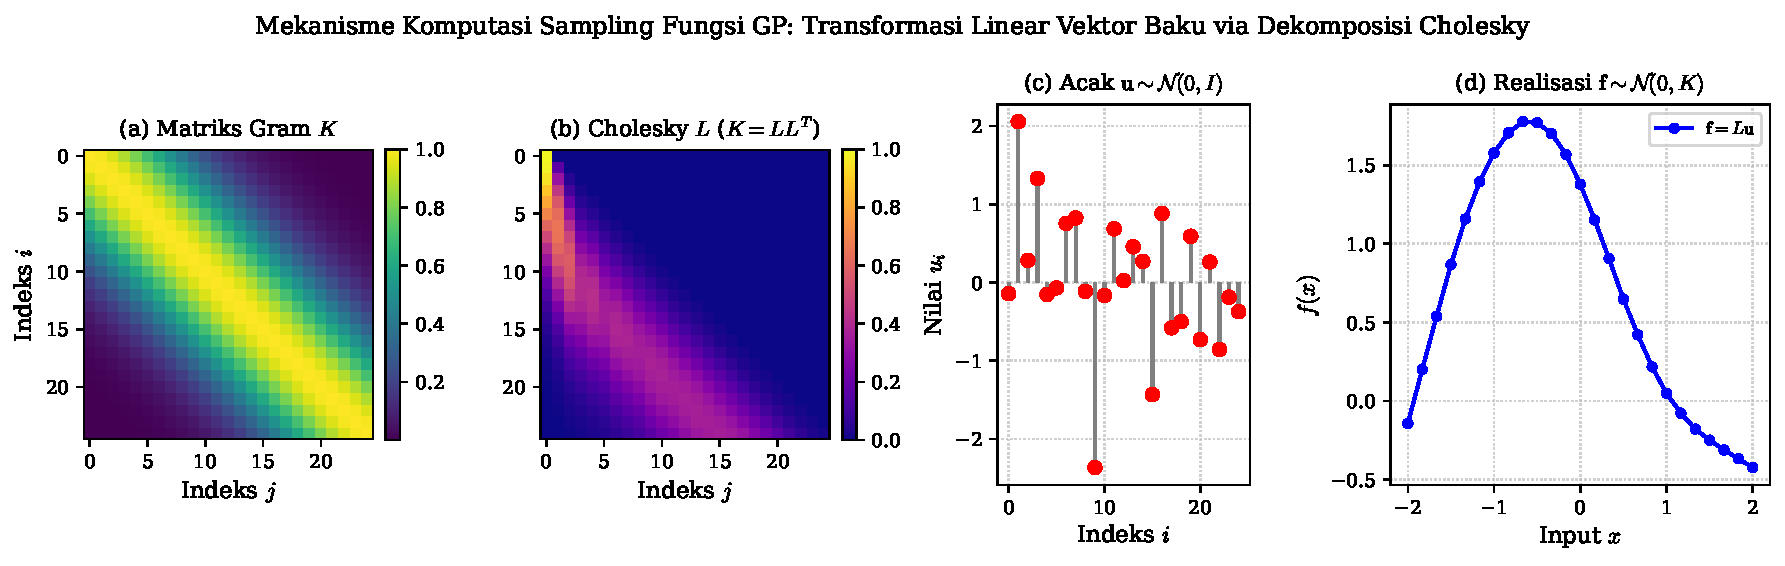
\includegraphics[width=0.95\textwidth]{fig4_cholesky_sampling_workflow.pdf}
\caption{Visualisasi alur kerja komputasi sampling fungsi: (a) Matriks kovariansi Gram $K$; (b) Faktor segitiga bawah Cholesky $L$; (c) Pembangkitan derau acak independen $\mathbf{u} \sim \mathcal{N}(\mathbf{0}, I)$; (d) Realisasi kurva fungsi halus hasil transformasi linear $\mathbf{f} = L\mathbf{u}$.}
\label{fig:cholesky_workflow}
\end{figure}

\subsection{Prosedur Sampling Langkah demi Langkah Beserta Alasannya}

Secara komputasional, proses pengambilan sampel dari distribusi Gaussian Process dieksekusi melalui lima tahapan berikut:

\begin{enumerate}
    \item \textbf{Langkah 1: Diskritisasi Domain Input ($X_*$)}
    \begin{itemize}
        \item \textit{Tindakan}: Menentukan $N_*$ titik koordinat evaluasi pada domain input yang tersusun rapat, $X_* = [\mathbf{x}_{*1}, \dots, \mathbf{x}_{*N_*}]^T \in \mathbb{R}^{N_* \times D}$.
        \item \textit{Alasan}: Komputer tidak dapat mengevaluasi domain kontinu secara tak hingga titik, sehingga fungsi diwakili oleh sampel titik diskret berkepadatan tinggi.
    \end{itemize}

    \item \textbf{Langkah 2: Evaluasi Matriks Kovariansi ($K = k(X_*, X_*)$)}
    \begin{itemize}
        \item \textit{Tindakan}: Menghitung nilai kernel $K_{ij} = k(\mathbf{x}_{*i}, \mathbf{x}_{*j})$ untuk setiap pasangan titik uji.
        \item \textit{Alasan}: Matriks $K$ bertindak sebagai ``pemberi aturan korelasi''. Pasangan titik yang berjarak sangat dekat memiliki nilai kovariansi mendekati $\sigma_f^2$ (dipaksa bernilai mirip), sedangkan titik yang berjauhan memiliki kovariansi mendekati 0.
    \end{itemize}

    \item \textbf{Langkah 3: Stabilisasi Numerik dan Dekomposisi Cholesky}
    \begin{itemize}
        \item \textit{Tindakan}: Menambahkan konstanta kestabilan (\textit{jitter}) $\tilde{K} = K + \epsilon_{\text{jitter}} I_{N_*}$ ($\epsilon_{\text{jitter}} = 10^{-6}$), kemudian menghitung matriks segitiga bawah $L = \operatorname{cholesky}(\tilde{K})$.
        \item \textit{Alasan}: Dekomposisi Cholesky memiliki kompleksitas komputasi yang sangat efisien ($\frac{1}{3}N_*^3$ FLOPs) dan hanya terdefinisi pada matriks definit positif. Penambahan \textit{jitter} mencegah kegagalan dekomposisi akibat galat pembulatan floating-point pada matriks dengan kondisi buruk (\textit{ill-conditioned}).
    \end{itemize}

    \item \textbf{Langkah 4: Pembangkitan Vektor Keacakan Murni ($\mathbf{u}$)}
    \begin{itemize}
        \item \textit{Tindakan}: Mengambil $N_*$ bilangan acak independen $\mathbf{u} \sim \mathcal{N}(\mathbf{0}, I_{N_*})$.
        \item \textit{Alasan}: Vektor $\mathbf{u}$ menyediakan variasi stokastik murni. Setiap sampel kurva baru yang ingin dibuat cukup dibangkitkan dari vektor $\mathbf{u}$ acak yang baru.
    \end{itemize}

    \item \textbf{Langkah 5: Transformasi Linear ($\mathbf{f} = \mathbf{m} + L \mathbf{u}$)}
    \begin{itemize}
        \item \textit{Tindakan}: Mengalikan matriks segitiga bawah $L$ dengan vektor acak $\mathbf{u}$ dan menambahkan vektor mean $\mathbf{m}$.
        \item \textit{Alasan}: Operasi perkalian matriks $L\mathbf{u}$ berfungsi mengikat (*mixing*) variabel-variabel acak independen tadi dengan bobot-bobot kovariansi pada baris matriks $L$, sehingga menghasilkan realisasi kurva yang kontinu dan mulus.
    \end{itemize}
\end{enumerate}

\subsection{Sampling Prior versus Sampling Posterior}

Mekanisme sampling di atas berlaku identik baik untuk distribusi sebelum observasi data (\textbf{Prior}) maupun sesudah observasi data (\textbf{Posterior}):

\begin{itemize}
    \item \textbf{Sampling Prior}:
    Menggunakan $\mathbf{m}_* = \mathbf{0}$ dan matriks kovariansi $K_* = K(X_*, X_*)$. Seluruh sampel fungsi berfluktuasi bebas di dalam pita ketidakpastian seragam $\pm 2\sigma_f$.
    \item \textbf{Sampling Posterior} (Terkondisi pada data training $\mathcal{D} = \{(x_i, y_i)\}_{i=1}^N$):
    Menggunakan mean prediktif $\bar{\mathbf{f}}_*$ dan matriks kovariansi prediktif $\Sigma_*$:
    \begin{align}
    \bar{\mathbf{f}}_* &= K(X_*, X) \left[ K(X, X) + \sigma_n^2 I_N \right]^{-1} \mathbf{y} \\
    \Sigma_* &= K(X_*, X_*) - K(X_*, X) \left[ K(X, X) + \sigma_n^2 I_N \right]^{-1} K(X, X_*)
    \end{align}
    Faktorisasi Cholesky diterapkan pada kovariansi prediktif: $L_{\text{post}} = \operatorname{cholesky}(\Sigma_* + \epsilon I)$. Sampel posterior dihitung melalui:
    \begin{equation}
    \mathbf{f}_{*,\text{post}}^{(s)} = \bar{\mathbf{f}}_* + L_{\text{post}} \mathbf{u}^{(s)}
    \end{equation}
    Pada lokasi titik di dekat training data, variansi pada $\Sigma_*$ bernilai mendekati nol ($L_{\text{post}} \approx \mathbf{0}$), sehingga seluruh realisasi sampel fungsi terkunci rapat dan dipaksa melewati nilai target observasi $y_i$.
\end{itemize}

\begin{figure}[h!]
\centering
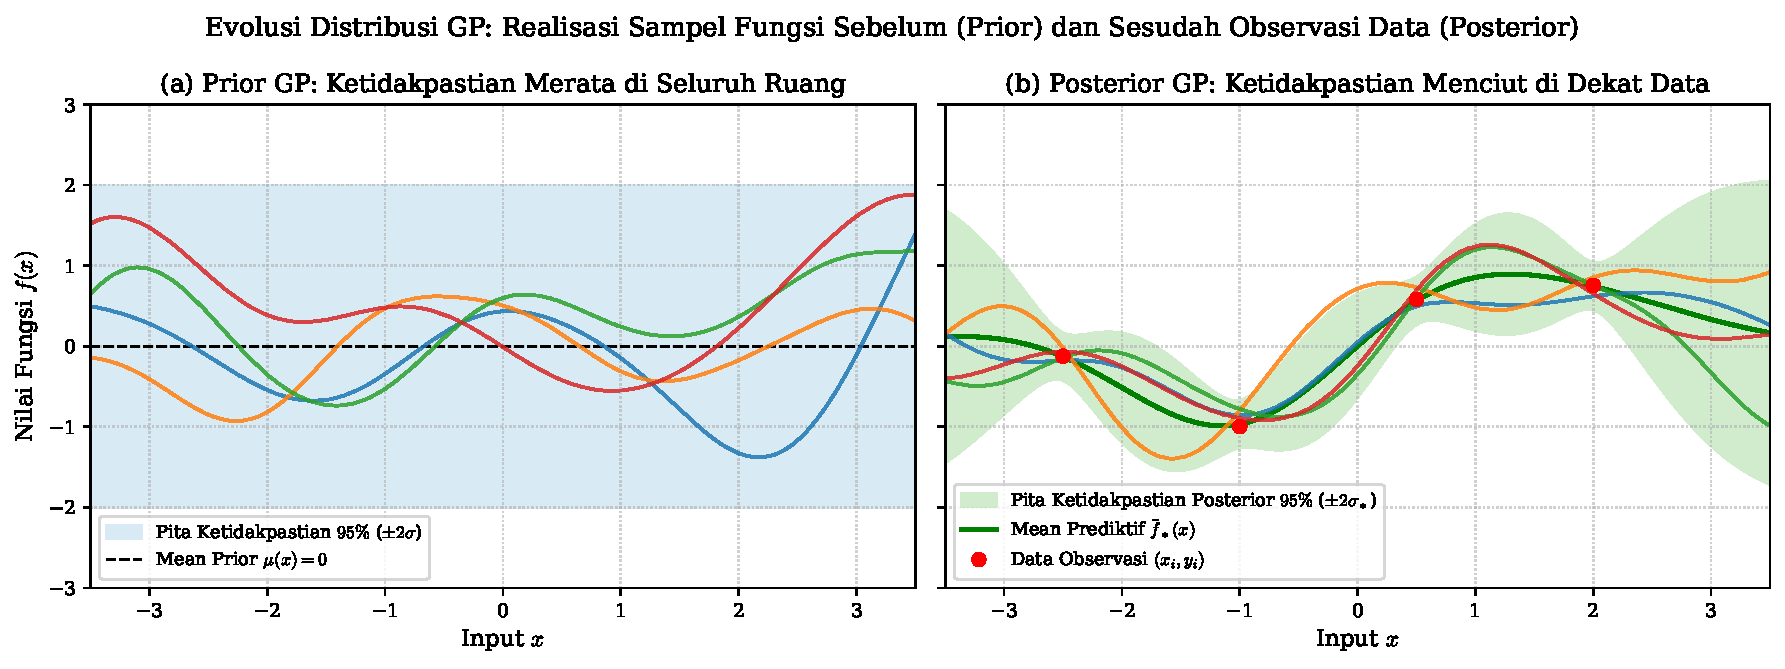
\includegraphics[width=0.95\textwidth]{fig5_prior_vs_posterior_samples.pdf}
\caption{Evolusi realisasi sampel fungsi: (Kiri) Sampel prior berosilasi bebas dengan ketidakpastian merata; (Kanan) Sampel posterior terkonsentrasi rapat mengikuti data observasi training.}
\label{fig:prior_posterior_samples}
\end{figure}

\subsection{Analisis Kestabilan Numerik dan Penanganan \textit{Jitter}}

Pada kernel stasioner dengan kehalusan tinggi ($C^\infty$) atau evaluasi grid padat, jarak antar titik evaluasi tetangga sangat kecil ($|x_i - x_{i+1}| \to 0$). Akibatnya, baris-baris pada matriks $K$ menjadi hampir linier dependen (\textit{nearly collinear}), menyebabkan rasio nilai eigen ekstrim ($\kappa(K) = \lambda_{\max}/\lambda_{\min} \gg 10^{12}$).

Galat pembulatan floating-point IEEE 754 dapat memicu nilai eigen terkecil secara semu menjadi nol atau negatif ($\lambda_{\min} \le 0$). Penambahan suku regularisasi diagonal (\textit{jitter}) $\epsilon_{\text{jitter}} I$ secara matematis menggeser seluruh spektrum nilai eigen:
\begin{equation}
\lambda_i(\tilde{K}) = \lambda_i(K) + \epsilon_{\text{jitter}} > 0
\end{equation}
Hal ini menjamin matriks tetap berstatus definit positif secara numerik tanpa mengubah korelasi spasial antar titik yang berbeda. Nilai $\epsilon_{\text{jitter}} \in [10^{-6}, 10^{-4}]$ terbukti optimal dalam menjaga stabilitas komputasi.

% =========================================================================
% BAGIAN 3: JEMBATAN MENUJU DEEP GAUSSIAN PROCESS & SEGMENTASI CITRA
% =========================================================================
\section{Keterbatasan Kernel Stasioner dan Motivasi Deep Gaussian Process}
\label{sec:dgp_motivation}

Analisis pada bagian sebelumnya menunjukkan bahwa kernel stasioner standar memaksakan asumsi ketergantungan spasial yang seragam di seluruh ruang input. Pada tugas segmentasi citra (\textit{Image Segmentation}), karakteristik ini menghadapi tantangan fundamental:

\begin{enumerate}
    \item \textbf{Ketidakseragaman Spasial (\textit{Spatial Non-Stationarity})}:
    Citra terdiri dari wilayah latar homogen berdampingan dengan tepi objek tajam (\textit{sharp object edges}). Kernel stasioner tunggal memicu fenomena \textit{over-smoothing}, di mana batas segmen piksel menjadi kabur.
    \item \textbf{Arsitektur Deep Gaussian Process (DGP)}:
    Untuk memodelkan fungsi non-stasioner tanpa merancang kernel manual yang rumit, DGP menyusun hirarki komposisi proses stokastik laten:
    \begin{equation}
    \mathbf{y} = f_L\big(f_{L-1}(\dots f_1(\mathbf{x})\dots)\big), \quad \text{dengan } f_\ell \sim \mathcal{GP}(m_\ell, k_\ell)
    \end{equation}
    Lapisan-lapisan GP laten awal bertindak sebagai transformasi non-linear ruang input (\textit{input space warping}), mentranslasikan koordinat spasial piksel menjadi representasi manifold laten non-stasioner sebelum dievaluasi pada lapisan klasifikasi segmentasi.
    \item \textbf{Propagasi Ketidakpastian via Sampling}:
    Inferensi pada DGP mengandalkan propagasi sampel fungsi antar lapisan laten via faktorisasi Cholesky dan aproksimasi variasional (\textit{Variational Inference}), menjadikan pemahaman sampling fungsi sebagai kunci utama implementasi sistem.
\end{enumerate}

% =========================================================================
% DAFTAR PUSTAKA
% =========================================================================
\begin{thebibliography}{99}
\bibitem{rasmussen2006gaussian}
Rasmussen, C. E., \& Williams, C. K. (2006). \textit{Gaussian Processes for Machine Learning}. MIT Press, Cambridge, MA.

\bibitem{damianou2013deep}
Damianou, A., \& Lawrence, N. D. (2013). Deep Gaussian Processes. \textit{Proceedings of the 16th International Conference on Artificial Intelligence and Statistics (AISTATS)}, PMLR 31:207-215.

\bibitem{salimbeni2017doubly}
Salimbeni, H., \& Deisenroth, M. (2017). Doubly Stochastic Variational Inference for Deep Gaussian Processes. \textit{Advances in Neural Information Processing Systems (NeurIPS)}, 30.
\end{thebibliography}

\end{document}
